\documentclass[a4paper, 12pt]{article}
%--------------------------------------
% Abstände
%--------------------------------------
\usepackage[left=30mm,right=20mm,top=25mm,headsep=15mm]{geometry}
\usepackage[onehalfspacing]{setspace}
%--------------------------------------
% encoding
%--------------------------------------
\usepackage[utf8]{inputenc}
\usepackage[T1]{fontenc}
%--------------------------------------
% German-specific commands
%--------------------------------------
\usepackage[ngerman]{babel}
%--------------------------------------
% Hyphenation rules
%--------------------------------------
\usepackage{hyphenat}
\hyphenation{Mathe-matik wieder-gewinnen} %Überflüssig?
%--------------------------------------
% Hyperlinks
%--------------------------------------
\usepackage{url}
\usepackage{hyperref}
%--------------------------------------
% Grafiken
%--------------------------------------
\usepackage[rightcaption]{sidecap}
\usepackage{graphicx}
\graphicspath{{images/}}
%--------------------------------------
% Kopf-& Fußzeile
%--------------------------------------
\usepackage{color}
\definecolor{fzp}{rgb}{0.565,0.612,0.671}
\usepackage{fancyhdr}
\setlength{\headheight}{37.9pt}
\pagestyle{fancy}
\fancyhf{}
%Kopfzeile links bzw. innen
\fancyhead[L]{\small{Leipzig - Ettlingen - Passau}}
%Kopfzeile mittig
\fancyhead[C]{}
%Kopfzeile rechts bzw. außen
\fancyhead[R]{
\includegraphics{FZP_RGB2.png}}
%Linie oben
%\renewcommand{\headrulewidth}{2pt}
\renewcommand\headrule
{{\color{fzp}%
	\hrule height 3pt width \headwidth
	\vspace{1pt}%
	\hrule height 1pt width \headwidth
	\vspace{-4pt}
}}
%Fußzeile rechts
\fancyfoot[R]{\thepage}
%Fußzeile Plain
\fancypagestyle{plain}{ %
  \fancyhf{} % remove everything
  \renewcommand{\headrulewidth}{0pt} % remove lines as well
  \renewcommand{\footrulewidth}{0pt}
  \renewcommand{\headrule}{}
  \fancyfoot[R]{\thepage}
}
%--------------------------------------
% Quellenverzeichnis 
%--------------------------------------
\usepackage[backend=biber,defernumbers,sorting=none,firstinits=true]{biblatex}
\addbibresource{biblo.bib}
%--------------------------------------
\begin{document}
%--------------------------------------
% großzügige Formatierungsweise
%--------------------------------------
\sloppy
%--------------------------------------
% Deckblatt
%--------------------------------------
\thispagestyle{empty}
\begin{center}
\Large{Berufliche Studienakademie Sachsen}
\end{center}
 
\begin{center}
\Large{Fachbereich Informatik}
\end{center}
\hspace{4cm}

\begin{center}
\textbf{\LARGE{Praxisarbeit}}
\end{center}
\hspace{4cm}

\begin{flushleft}
\begin{tabular}{l p{10pt} p{290pt}}
& & \textbf{im Studiengang Informatik}\\
\\
\textbf{Thema:} & &  Biometrische Unterschrift in einem mittelständischen Unternehmen 
der Vermietungsbranche zur personalisierten Warenabgabe.\\
& & \\
& & \\
& & \\
\textbf{eingereicht von:} & & Sebastian Kloppe \\
& &                           Braustraße 17 - 19\\
& &                           04107 Leipzig\\
& & \\
\textbf{Seminargruppe:} & & CS13-2 \\
\textbf{Matrikelnummer:} & & 5000349\\
& & \\
& & \\
\textbf{Betreuer:} & & B.Sc. Benjamin Teßmar\\
& &                    Funk, Zander \& Partner GmbH\\
& &                    Kreuzstraße 7\\
& &                    04103 Leipzig\\
& & \\
& & \\
& & \\
& & \\
& & \\
& & \\
& & \\
\textbf{eingereicht am:} & & 11. Juli 2014 in Leipzig\\
\end{tabular}
\end{flushleft}
%--------------------------------------
% Inhaltsverzeichnis
%--------------------------------------
\newpage
%\thispagestyle{plain}
\pagenumbering{Roman}
\tableofcontents
%--------------------------------------
% Abbildungsverzeichnis
%--------------------------------------
\newpage
%\thispagestyle{plain}
\listoffigures

\newpage
%--------------------------------------
% Einleitung
%--------------------------------------
\clearpage 
\pagenumbering{arabic}   

\section{Einleitung}
\label{sec:Einleitung}
Das Unternehmen, die Funk, Zander \& Partner GmbH, hat sich seit der Gründung im Jahr 1992 auf die elektronische Datenverarbeitung und Unternehmensberatung spezialisiert. Das weitere Unternehmensangebot umfasst anwenderbezogene Schulungen und Programmierungsarbeiten. Das Thema "'Biometrische Unterschrift"' ist im Rahmen einer Softwareumstellung eines Kunden entstanden. Aus diesem Grund wurde am 16. April 2014 bei Herrn Prof. Dr. Brunner das oben genannte, abweichende Thema für die Praxisarbeit beantragt und genehmigt.


\subsection{Motivation}
\label{subsec:Motivation}
Unser Auftraggeber ist ein inhabergeführtes, mittelständisches Unternehmen und angewiesen, aufgrund zunehmender Komplexität der Unternehmensprozesse sowie steigender Auftragszahlen, dass bestehende System zur Auftrags- und Materialverwaltung sowie der Kundendatenverwaltung auf Grundlage von MS-DOS durch die Sage Office Line, einer vollständigen ERP-Lösung\footnote{\label{foot:1}Enterprise-Resource-Planning: Effizente Planung / Steuerung von Unternehmensressourcen. \cite{ERP}}, der Firma Sage Software GmbH (Sage) sowie durch Zusatzmodule der Firma Funk, Zander \& Partner GmbH (FZP) abzulösen, um wettbewerbsfähig zu bleiben. \cite{einleitung1}

\subsection{Zielsetzung}
\label{subsec:Zielsetzung}
Im Zuge der Softwareumstellung wird angestrebt die Warenabgabe mittels biometrischer Signatur auf Lieferscheinen und Rechnungen zu personalisieren. Desweiteren entsteht ein Nachweis über die erbrachten Lieferungen und Leistungen. Hierfür wird eine Schnittstellenlösung von FZP mit Hilfe eines Signatur-Tablets der Firma Wacom entwickelt. Die neu geschaffene Schnittstelle reicht die erfassten Daten an eine bestehende Schnittstelle von FZP zur Erstellung von Vermietungsbelegen weiter. \cite{einleitung1}
%--------------------------------------
% Grundlagen
%--------------------------------------
\section{Grundlagen}
\label{sec:Grundlagen}
Die ersten Überlegungen und gesetzlichen Regelungen zum Thema "'Biometrische Merkmale"' begannen bereits durch
das sogenannte Volkszählungsurteil des Bundesverfassungsgerichts vom 15. Dezember 1983, welches besagt, dass
die Bürger grundsätzlich ein Selbstbestimmungsrecht über die Vergabe und Verwendung ihrer Daten besitzen.
Dies gilt als Meilenstein des Datenschutzes. Dadurch wurde das informationelle Selbstbestimmungsrecht als
Grundrecht gemäß Art. 2 Abs. 1 in Verbindung mit Art. 1 Abs. 1 des Grundgesetzes festgelegt. Auf europäischer Ebene wurde dies mit Art. 8 Abs. 1 der Europäischen Menschenrechtskonvention fixiert. \cite{grundlagen1}\cite{grundlagen2}\cite{grundlagen3} Mit dem Informations - und Kommunikationsdienste - Gesetz (IuKDG)\footnote{\label{foot:2} BGBl. I S. 1870,
1872 ff. vom 22. Juli 1997 \cite{grundlagenFN1}} wurde 1997 die erste gesetzliche Regelung zur elektronischen
Signatur veröffentlicht. Im Jahr 2001 ist das Gesetz über Rahmenbedingungen für elektronische Signaturen (SigG)\footnote{\label{foot:3} BGBl. I S. 876. vom 16. Mai 2001 \cite{grundlagenFN2}} als Nachfolger des IuKDG in Kraft getreten und wird stetig anhand neuer gesetzlicher Regelungen aktualisiert. \cite{grundlagen4}

\subsection{Stand des Wissens}
\label{sec:Stand des Wissens}
Grundsätzlich unterscheidet man zwischen dem Begriff "'Digitale Signatur"' als Verfahren zur Verschlüsselung von Daten und "'Elektronische Unterschrift"' als Verfahren zur Erfassung der Daten für das Verschlüsselungsverfahren. Unter "'Biometrischer Unterschrift"' versteht man eine "'Elektronische Unterschrift"' verknüpft mit biometrischen Daten des Unterschriftgebers.
\newline
Die Gesetze IuKDG und SigG sind zum Schutz der Anwender und Nutzer geschaffen wurden. Diese dienen zur Gewährleistung von Vertraulichkeit, Verfügbarkeit und Zurechenbarkeit der Teilnehmer am Signaturverfahren. \cite{standdeswissens1} Als Hauptaufgabe des SigG zählt die Prüfung von Integrität und Authentizität der Kommunikationspartner. Die Garantie der Unversehrtheit des Dokuments und des Inhalts können als weitere Ziele genannt werden. Die "'Elektronische Unterschrift"' dient ebenfalls als Beweismittel vor Gericht. Im Signaturverfahren wird zwischen den nachfolgenden vier Beteiligten unterschieden. \cite{standdeswissens2}

\subsubsection{Nutzer / Anwender}
\label{sec:Nutzer / Anwender}
Laut \S 2 Nr. 9 SigG kann ein Nutzer bzw. Antragsteller auf die Ausfertigung einer digitalen Signatur nur eine natürliche Person sein. Eine juristische Person in Form einer Gesellschaft mit beschränkter Haftung (GmbH) oder einer Aktiengesellschaft (AG) darf dadruch nicht als Nutzer von digitalen Signaturen direkt auftreten. Der Grund hierfür ist, dass eine GmbH oder eine AG durch mehrere natürliche Personen, wie dem Aufsichtsrat, Vorstand oder mehreren Geschäftsführern, vertreten werden kann. Eine eindeutige Identifikation und Authentikation des Nutzers der digitalen Signatur ist infolgedessen nicht mehr möglich. Andererseits besteht die Möglichkeit, dass eine natürliche Person die Nutzung seines Signaturschlüssels für weitere natürliche Personen autorisiert und entsprechend des Signaturgesetzes beispielsweise mehrere Geschäftsführer einer GmbH mit einem Signaturschlüssel auftreten können. Des Weiteren ist es dem Signaturschlüssel-Inhaber möglich zusätzliche Informationen gemäß \S 5 Abs. 2 SigG in Form eines Attribut-Zertifikates zu hinterlegen. In einem Attribut-Zertifikat können Vertretungsvollmachten für dritte Personen, berufsrechtliche Zulassung und sonstige Angaben zur Person eingetragen werden. Außerdem besteht eine Verpflichtung gegenüber dem Nutzer von digitalen Signaturen, den privaten Schlüssel sorgfältig aufzubewahren. Die Aufbewahrung ist wichtig um den Gebrauch und die damit einhergehende Identitätsannahme des Signaturschlüssel-Inhabers von unbefugten Personen zu verhindern. Der private Schlüssel ist meistens auf einer Chipkarte hinterlegt und vor Veränderungen geschützt. \cite{standdeswissens3}\cite{standdeswissens4}

\subsubsection{Zertifizierungstelle / Trustcenter}
\label{sec:Zertifizierungstelle / Trustcenter}
Laut \S 2 Nr. 8 SigG können Zertifizierungsstellen von natürlichen und juristischen Personen betrieben werden. Der Betrieb einer Zertifizierungsstelle ist grundsätzlich genehmigungsfrei, obliegt dennoch folgenden Bestimmungen nach \S 4 SigG. Der Betrieb einer Zertifizierungsstelle setzt Fachkunde, Zuverlässigkeit, Deckungsvorsorge gemäß \S 12 SigG gegen Schadenersatzansprüche voraus. Des Weiteren ist die Erfüllung der Sicherheitsansprüche anhand eines von der Prüfstelle abgenommenen Sicherheitskonzepts notwendig. "'Die erforderliche Fachkunde liegt vor, wenn die im Betrieb eines Zertifizierungsdienstes tätigen Personen über die für diese Tätigkeit notwendigen Kenntnisse, Erfahrungen und Fertigkeiten verfügen"' \footnote{\S 4 Abs. 2 Satz 3 Signaturgesetz \cite{grundlagenFN2}}. "'Die erforderliche Zuverlässigkeit besitzt, wer die Gewähr dafür bietet, als Zertifizierungsdiensteanbieter die für den Betrieb maßgeblichen Rechtsvorschriften einzuhalten"' \footnote{\S 4 Abs. 2 Satz 2 Signaturgesetz \cite{grundlagenFN2}}. Als Trust Center bezeichnet man die Einrichtungen, die die Verschlüssung von Daten anbieten und das Hochsicherheitsrechenzentrum betreiben. Zertifizierungsstellen und Trust Center werden benötigt, wenn eine große Anzahl von Benutzern am digitalen Signaturverfahren teilnehmen. Die Hauptaufgabe der Zertifizierungsstelle ist die Identifizierung der Antragssteller für einen Signaturschlüssel mittels Personalausweis sowie die Vergabe und Zuordnung der öffentlichen Signaturschlüssel. Des Weiteren sichern sie die Authentizität des Absenders im Rechtsverkehr, vergleichbar mit einer amtlichen Beglaubigung von Behörden und Notaren. \cite{standdeswissens3}\cite{zertstelle1} 
\begin{figure}[!ht]
    \centering
    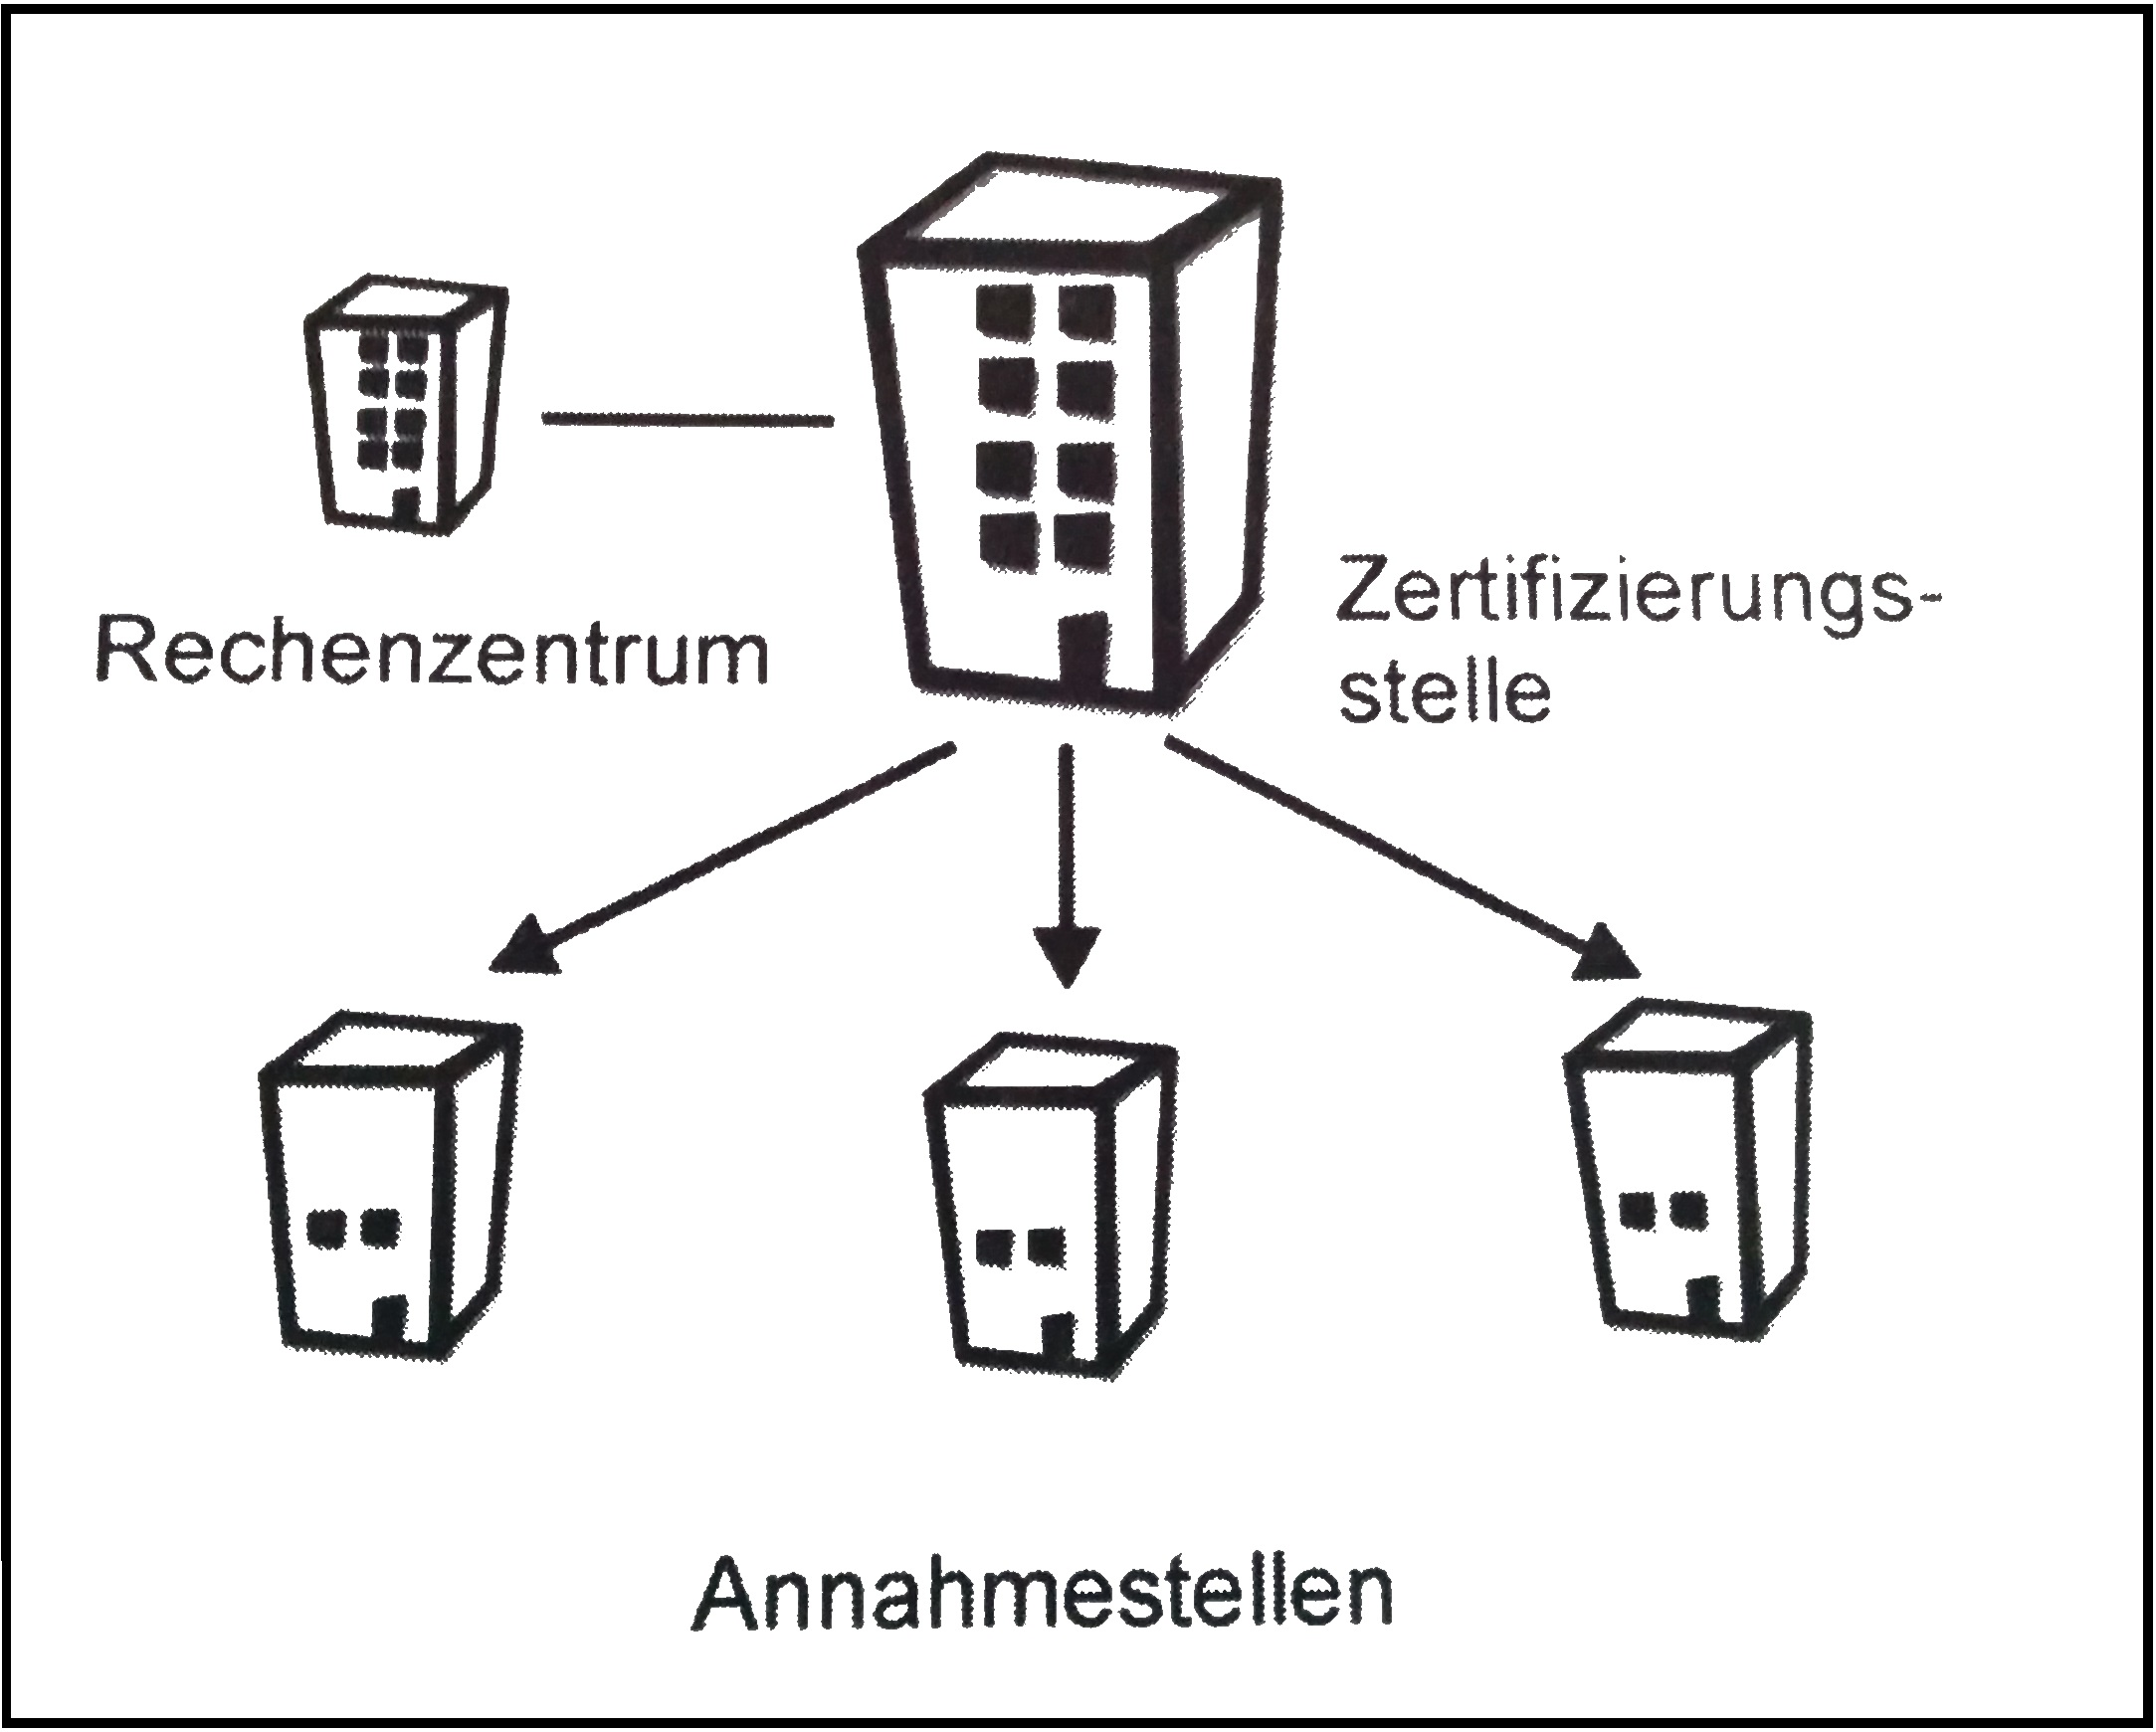
\includegraphics[height=230pt, width=280pt]{trustcenterNeu3.jpg}
    \caption[Schema einer Zertifizierungsstelle]{\small{Schema einer Zertifizierungsstelle \cite{trust1}}}
\end{figure}
\newline
\pagebreak
\textbf{} %Workaround
\newline
Wie auf der Abbildung 1 zu sehen ist, lässt sich die Zertifizierungsstelle in zwei Bereiche einteilen. Auf der einen Seite steht die Annahmestelle, welche die Identifikation der Antragsteller mit Personalausweis und weiteren notariell beglaubigten Dokumenten, z.B. Zulassungen übernehmen. Auf der anderen Seite steht die Zertifizierungsstelle, welche die Erzeugung der Schlüsselpaare und Zertifikate übernimmt. Die Zertifizierungsstelle muss sicherstellen, dass niemand den privaten Schlüssel modifizieren kann. Weiterhin muss der Dienst zur Prüfung der digitalen Signaturen immer verfügbar sein. Abgesehen davon muss sichergestellt werden, dass nur der Antragsteller den privaten Schlüssel erhält. Dies wird meistens mit Chipkarten realisiert. Auf den Chipkarten befindet sich der private Schlüssel und ist vor Auslesung, Manipulation oder Löschung geschützt. Zusätzlich müssen Zertifizierungsstellen noch Dienste, wie die Zulassung von Pseudonyme zur Wahrung des Personlichkeitsrechts des Schlüsselinhabers und ein 24-Stunden-Sperrdienst für Signaturschlüssel anbieten. Des Weiteren muss die Schlüsselaufbewahrung vom Auftraggeber ausdrücklich erklärt werden, ansonsten ist die Speicherung von privaten Schlüsseln in Zertifizierungsstellen nicht erlaubt. Die Pflege des Schlüsselverzeichnis ist von besonderer Bedeutung, da jederzeit die Identifikation von Kommunikationspartnern möglich sein muss. Das Schlüsselverzeichnis muss ständig aktuell und funktionstüchtig sein. Ein weiterer Dienst ist der Zeitstempeldienst. Dieser dient zur genauen Festhaltung, wann ein Dokument erzeugt, verändert oder gelöscht wurde, mittels Zeitangabe der Zertifizierungsstelle im Hashwert für das signierte Dokument. Anwendung findet dieses Verfahren bei der Einhaltung von gesetzlichen Fristen und der Festlegung von Gültigkeitsdauern. \cite{standdeswissens3}\cite{zertstelle1}

\subsubsection{Pr"ufstelle}
\label{sec:Pr"ufstelle}
Die Prüfstelle ist zur Prüfung des Sicherheitskonzeptes der Zertifizierungsstelle beauftragt und benötigt die Anerkennung der Regulierungsbehörde. Die Aufgabe der Prüfstelle ist die Kontrolle und Abnahme der Hard- und Softwarekomponenten gemäß dem Signaturgesetz. Der Prüfbericht wird anschließend von der Regulierungsbehörde veröffentlicht. \cite{standdeswissens3}

\subsubsection{Regulierungsbeh"orde}
\label{sec:Regulierungsbeh"orde}
Die Regulierungsbehörde, auch Bundesnetzagentur (BNetzA) genannt, ist eine Bundesoberbehörde mit Sitz in Bonn, welche am 01.01.1998 als Nachfolgerin des Bundesministeriums für Post und Telekommunikation sowie der Deutschen Bundespost gegründet wurde. Die Kontrolle der Einhaltung der gesetzlichen Bestimmungen des Signaturgesetzes ist nur ein Bestandteil der Behörde, welche auch für das Wettbewerbsrecht der Telekommunikationsbranche zuständig ist. Die Hauptaufgaben der BNetzA im Signaturprozess liegt in der Vergabe / Entziehung der Genehmigungen für den Betrieb einer Zertifizierungsstelle, der Kontrolle der Zertifizierungsstellen sowie der Ausstellung eines Zertifikates, das die Zertifizierungsstelle authentisiert. \cite{standdeswissens3}\cite{regBeh1}

\subsection{Technologien}
\label{sec:Technologien}
Die wesentlichen Schritte im digitalen Signaturgsprozess sind das Signieren, Verschlüsseln und Prüfen mittels des asymmetrischen Schlüsselkonzeptes. Das asymmetrische Schlüsselkonzept besteht aus der Generierung eines öffentlichen Schlüssels, dieser wird in einer Zertifizierungsstelle hinterlegt und einem privaten Schlüssel, diesen besitzt der Signaturschlüssel-Inhaber, welcher auf einer Chipkarte vor Manipulationen geschützt ist und nicht verändert werden kann. \cite{techno1} 
\begin{figure}[!ht]
    \centering
    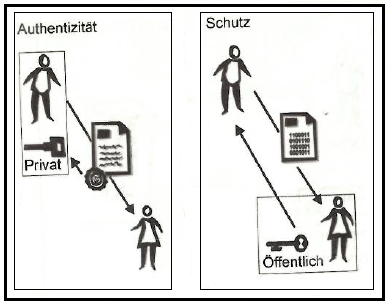
\includegraphics[height=260pt, width=350pt]{ablauf_async.PNG}
    \caption[Asymmetrisches Schlüsselkonzept]{\small{Asymmetrisches Schlüssel Konzept \cite{techno5}}}
\end{figure}

\subsubsection{Erstellung Dokumente}
\label{sec:Erstellung Dokumente}
Das asymmetrische Schlüssel Konzept geht auf das von Whitfield Diffie 
und Martin Hellmann im Jahr 1976 entwickelte Verschlüsselungsverfahren 
DH76 zurück. In dem Verfahren werden 2 voneinander abhängige Schlüssel 
generiert. Ein Schlüssel dient zur Verschlüsselung und ist geheim. Der 
andere Schlüssel wird zur Entschlüsselung verwendet und ist öffentlich. 
Die digitale Signatur dient vorrangig nicht der Unkenntlichmachung der 
Dokumente und Information, sondern der Feststellung, ob die signierten 
Informationen unversehrt bei dem Empfänger angekommen sind oder verändert 
wurden sowie zur Identifizierrung des Signaturschlüssel-Inhabers. Die 
Prüfung auf Echtheit des Signaturschlüssels wird mit dem öffentlichen 
Schlüssel übernommen. Der private Schlüssel signiert nicht das gesamte 
Dokument, sondern nur einen repräsentativen Bereich. \cite{techno1}
\begin{figure}[!ht]
    \centering
    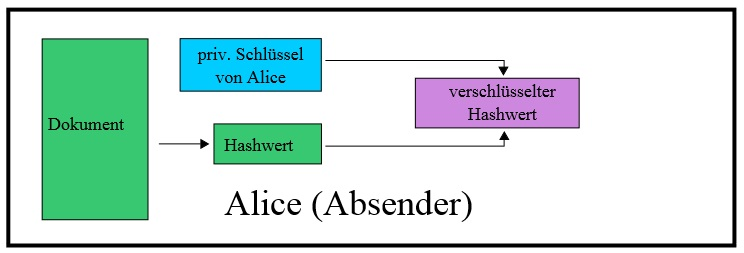
\includegraphics[width=\textwidth]{ErstellungAbsender2.jpg}
    \caption[Erstellung eines Dokuments mit digitaler Signatur]{\small{Erstellung eines Dokuments mit digitaler Signatur. \cite{techno3}}}
    \label{fig:2}
\end{figure}\\
Der erste Schritt im Signierungsprozess ist das bilden eines Fingerabdrucks (Hashwert) des Dokuments. Der Fingerabdruck wird mittels Hash-Algorithmus von einem Teil des Dokuments erstellt und ist mit hoher Wahrscheinlichkeit eindeutig. Ein Hash-Algorithmus ist eine mathematische Funktion, die eine beliebig große Menge an Eingabewerten möglichst gleichmäßig auf eine eingeschränkte Ausgabemenge abbildet. \cite{techno2} Eine absolute Eindeutigkeit des Fingerabdrucks kann auf Grund des Zufallsprinzips bei Hash-Algorithmen nicht gewährleistet werden. Anhand des Fingerabdrucks kann nicht auf das Dokument geschlossen werden. Weiterhin ist die Erstellung des Dokuments aus dem Fingerabdruck nicht möglich, da der Hashwert von einem beliebigen Teil des Dokuments erstellt wird. Im zweiten Schritt des Prozesses wird der Fingerabdruck mittels privaten Signaturschlüssels zur Sicherstellung der Unversehrtheit des Dokuments verschlüsselt. Im letzten Schritt werden der verschlüsselte Fingerabdruck und das Dokument zu einer Datei vereint. \cite{techno1}   

\subsubsection{Biometrische Daten}
\label{sec:Biometrische Daten}
Neben der Erstellung eines Fingerabdrucks mittels Hash-Algorithmus, können der digitalen Signatur noch weitere Daten, wie biometrische Charakteristika des Signaturschlüssel-Inhabers angehängt werden. Die Biometrie setzt sich aus den Worten "bios" (Leben) und "métron" (Maßstab) zusammen und "'beschäftigt sich mit Messungen an Lebewesen und den dazu erforderlichen Mess- und Auswertungsverfahren"' \cite{bioMet1}. Ziel ist die Identifizierung sowie die Authentifizierung von Personen anhand deren einzigartiger und konstanter biometrischer Merkmale. Unter biometrischen Merkmalen versteht man unteranderem, dass Papillarmuster der Finger, die Handgeometrie und die Handlinien, die Vermessung des Gesichtes, die Iris- und Retinastruktur, die DNA, der Stimmabgleich, das Bewegungsmuster und die Unterschrift. Bei einer elektronischen Unterschrift mit biometrischen Merkmalen benötigt man hauptsächlich die Schreibgeschwindigkeit, den ausgeübten Druck, den Bereich und die Dauer der Unterschrift. Das Schriftbild dient ebenfalls zur Identifizierung und Authentifizierung einer Person. Andererseits ist eine 100 prozentige Genauigkeit bei biometrischen Merkmalen nicht gewährleistet. Zu Fehlern in den Mess- und Auswertungsverfahren kann es durch altersbedingte Veränderungen, Körperveränderungen, wie z. B. Verletzung oder Verlust von Gliedmaßen, der Veränderung der Iris kommen. Eine weitere Fehlerquelle entsteht durch Täuschung oder Manipulation von Prüfungsgeräten. \cite{bioMet2}\cite{bioMet3}

\subsubsection{Versendung Dokumente}
\label{sec:Versendung Dokumente}
Nach der Vereinigung der Komponenten werden der Dokumentendatei zusätzlich der öffentliche Signaturschlüssel sowie das Zertifikat des Signaturschlüssel-Inhabers angehängt und versendet. Anhand des Zertifikates kann die Identitätsprüfung des Absenders durchgeführt werden. Die Bestandteile des Zertifikates sind der Name bzw. das Pseudonym des Signaturschlüssel-Inhabers, die Zertifizierungsstelle und deren Identifizierungsnummer, das Ausstellungsdatum sowie die Gültigkeitsdauer und der öffentliche Signaturschlüssel mit dem verwendeten Hash-Algorithmus. \cite{techno1}\cite{techno4}
\begin{figure}[!ht]
    \centering
    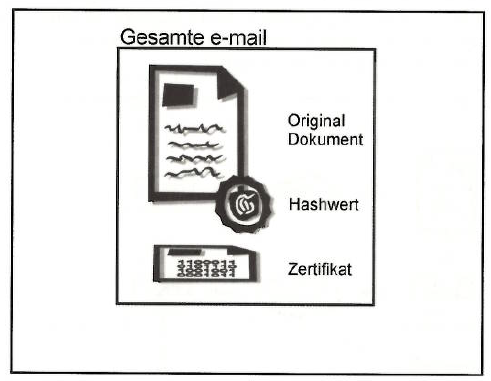
\includegraphics[height=220pt, width=300pt]{versand_doc.PNG}
    \caption[Aufbau versandfertiges Dokument]{\small{Aufbau versandfertiges Dokument \cite{techno6}}}
\end{figure}

\subsubsection{Pr"ufung Dokumente}
\label{sec:Pr"ufung Dokumente}
Die Prüfung des Dokuments erfolgt im ersten Schritt auf Echtheit des öffentlichen Schlüssels mittels der Identifizierungsnummer und des Namens der Zertifizierungsstelle aus dem übermittelten Zertifikat. Im nächsten Schritt wird die Prüfung des Zertifikates mithilfe des öffentlichen Schlüssels aus der öffentlich, zugänglichen Datenbank der Zertifizierungsstelle durchgeführt. Ist die Echtheit sichergestellt wird die Entschüsselung der Signatur durch den öffentlichen Schlüssel durchgeführt. Das Ergebnis der Entschlüsselung ist der vom Absender erzeugte Fingerabdruck. Als letzter Schritt wird anhand des im Zertifkat genannten Hash-Algorithmus erneut ein Fingerabruck des Dokuments erstellt und mit dem entschlüsselten Fingerabdruck verglichen. Die Unversehrheit des Dokuments ist gewährleistet, wenn die beiden Fingerabdrücke des Dokuments übereinstimmen. \cite{techno1}
\begin{figure}[!ht]
    \centering
    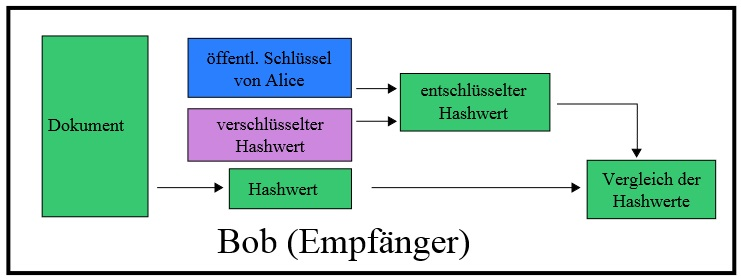
\includegraphics[width=\textwidth]{PruefungEmpfaenger2.jpg}
    \caption[Prüfung eines Dokuments mit digitaler Signatur]{Prüfung eines Dokuments mit digitaler Signatur. \cite{techno3}}
    \label{fig:3}
\end{figure}
%--------------------------------------
% Konzeption
%--------------------------------------
%\newpage
\section{Konzeption}
\label{sec:Konzeption}
\subsection{Einleitung}
Das mittelständige Unternehmen ist in den Bereichen Maschinenbau, Reparaturen und Instandsetzungen sowie Verkauf und Vermietung tätig. Die Produkte des Verkaufs und der Vermietung sind hochwertige Elektromaschinen sowie Werkzeuge und Verbrauchsmaterialien. Desweiteren werden Instandhaltungs- und Reparaturaufträge für Maschinen sowie Spezialanfertigung im Bereich Maschinenbau angeboten. Die Kundschaft besteht überwiegend aus selbstständigen Handwerkern, kleineren Betrieben und Angehörigen aus Land- und Forstwirtschaft. \cite{einleitung1}
\subsection{Ist-Zustand}
Die Warenabgabe im Verkauf und der Vermietung erfolgt in einem Ladengeschäft mittels handgeschriebener Rechnungen und Aufträge. Im nächsten Schritt werden die Aufträge und Rechnungen zur weiteren Verwendung in das bestehende MSDOS-System wiederholt händisch übertragen. Im darauffolgenden Schritt werden die handgeschriebenen Belege an die Buchhaltungsabteilung zur Prüfung des Rechnungseingangs und Rechnungsausgangs sowie an die Fertigungsabteilung zur Auftragsbearbeitung weitergereicht. \textbf{Screenshots vorhanden vom DOS System?} \cite{einleitung1}
\begin{figure}[!ht]
    \centering
    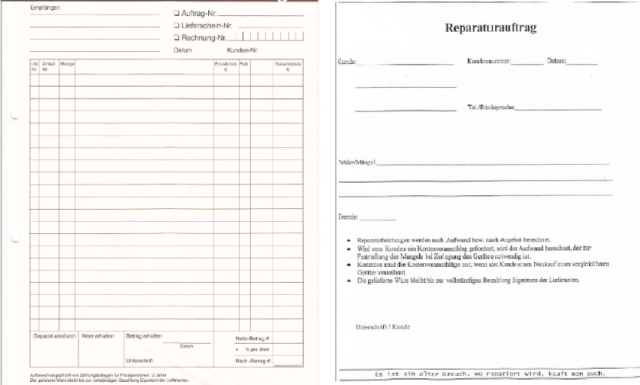
\includegraphics{rechnungReparaturAlt2.png}
    \caption[Muster Rechnungsvordruck und Reparaturauftrag]{Muster eines Rechnungsvordruck (li.) und Reparaturauftrag (re.) \cite{einleitung1}}
    \label{fig:4}
\end{figure}
\subsection{Ziele}
Das Hauptziel der Umstellung ist die Ablösung des bestehenden Altsystems und der daraus resultierenden Vereinfachung und Beschleunigung der Geschäftsprozesse. Die Entlastung der Mitarbeiter sowie die Kostenreduzierung und Effizienzsteigerung sind weitere Ziele. Das Ziel der personalisierten Warenabgabe ist der eindeutige Nachweis über die erbrachten Lieferungen und Leistungen sowie die rechtliche Absicherung gegenüber Dritten. Im Bereich Umsetzung werde ich hauptsächlich auf die personalisierte Warenabgabe mittels digitaler Signatur eingehen. \cite{einleitung1}
\subsection{Umsetzung}
Im ersten Schritt wurde die Anbindung der neu zuschaffenden Schnittstelle zur Erfassung der Daten aus dem Signatur-Tablet sowie die Weitergabe und Integration in den bestehenden Datenbestand der Sage Office Line durch FZP geprüft. Im zweiten Schritt wurden verschiedene Anbieter von Signatur-Tablets geprüft. Hier hat sich die Firma Wacom schnell heraus kristallisiert, wegen der Unternehmenserfahrungen seit 1983 \cite{konzept1} sowie der guten Anbindungen des grafischen Tablets mittels des bereit gestellten SDK\footnote{\label{foot:4} Software Development Kit: Sammlung von Werkzeugen und Anwendungen, um eine Software zu erstellen, meist inklusive Dokumentation. \cite{SDK}}. Nach Abschluss der Prüfungen wurde mit der Entwicklung der Schnittstelle begonnen. Der erste Schritt ist die Einbindung der benötigten DLL\footnote{\label{foot:5} Dynamic Link Library: Dynamische Programmbibliothek für Microsoft Betriebssysteme. \cite{DLL}} in das Entwicklungsprojekt. Die DLL umfassen unteranderen die benötigten Komponenten zur Kommunikation zwischen der Schnittstelle und der Sage Office Line sowie dem Signatur-Tablet. Desweiteren werden die DLL des Signatur-Tablets zur Erfassung und Prüfung der digitalen Signatur benötigt und eingebunden.

Die 

\subsection{Umsetzung}
\label{sec:Umsetzung}
Zu Beginn der Umsetzung wurde die Anbindung der neuzuschaffenden Erweiterung zur Erfassung der Daten aus dem Signatur-Tablet sowie die Weitergabe und Integration in den bestehenden Datenbestand der Sage Office Line durch FZP analysiert. Anschließend wurden verschiedene Anbieter von Signatur-Tablets geprüft. Hier hat sich die Firma Wacom schnell heraus kristallisiert, hinsichtlich der Unternehmenserfahrungen seit 1983 \cite{konzept1}. Ein weiteres positives Merkmal ist die guten Anbindung des grafischen Tablets mittels des bereit gestellten Software Developer Kits (SDK)\footnote{\label{foot:4}Software Development Kit: Sammlung von Werkzeugen und Anwendungen, um eine Software zu erstellen, meist inklusive Dokumentation. \cite{SDK}}. Nach Abschluss der Prüfungen wurde mit der Entwicklung der Erweiterung begonnen. Die Entwicklung von Zusatzmodulen und Erweiterungen ist angesichts des modularen Aufbaukonzepts der Sage Office Line möglich. Die Einbindung von Erweiterungen wird mit einer eigenentwickelten Methode von Sage, namens Dynamic Link Library\footnote{\label{foot:6}Dynamic Link Library: Dynamische Programmbibliothek für Microsoft Betriebssysteme. \cite{DLL}} (DLL) Common Method (DCM) realisiert. Mit dieser Methode können Anpassung an der Sage Office Line auf Basis des Microsoft .NET Frameworks\footnote{\label{foot:5}Framework: Grundstruktur / Rahmenwerk zur Bestimmung der 
Software-Architektur. Es besteht aus mehreren Klassen, die zusammenarbeiten und wieder verwendbare Entwürfe darstellen. \cite{framework}} vorgenommen werden. Mit Hilfe von DCM werden die Anpassungen mit der verwendeten Technologie der Sage Office Line auf Basis von Microsoft Access in Verbindung mit dem Microsoft Component Object Model Frameworks (COM) verbunden. Zuerst ist die Einbindung der benötigten DLLs in das Microsoft .NET Entwicklungsprojekt notwendig. Die DLLs umfassen unteranderen die benötigten Komponenten zur Kommunikation zwischen der Erweiterung, der Sage Office Line und dem Signatur-Tablet. Des Weiteren werden die DLLs des Signatur-Tablets zur Erfassung und Prüfung der biometrischen Unterschrift eingebunden. Das Entwicklungsprojekt ist in die Projekte "'FZP.OfficeLine.Abf.Signatur"' und "'FZP.Wacom"' unterteilt. Die Aufteilung in Unterprojekte wurde angesichts der Wiederverwendbarkeit von einzelnen Projektteilen gewählt.
\begin{figure}[!ht]
    \centering
    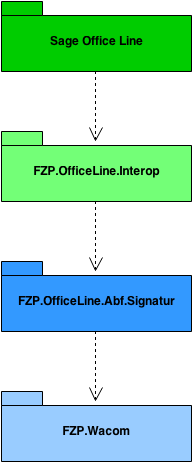
\includegraphics[height=260pt, width=130pt]{paketDiagrammNeu2.png}
    \caption[Paketdiagramm FZP.Wacom.Erweiterung]{\small{Paketdiagramm FZP.Wacom.Erweiterung}}
\end{figure}
\newline
Das in der nächsten Seite dargestellte Klassendiagramm symbolisiert das Projekt "'FZP.OfficeLine.Abf.Signatur"'. Der rot umrandete Bereich zeigt die Klassen, die die Anbindung an die Sage Office Line regeln. Es existieren zwei Klassen, welche die Erfassungsmaske für die biometrische Unterschrift aus der Sage Office Line heraus öffnen können. Die Erfassungsmaske kann im Standard des Verkaufsbereichs der Sage Office Line sowie im Zusatzmodul FZP Vermietung gestartet werden.
\begin{figure}[!ht]
    \centering
    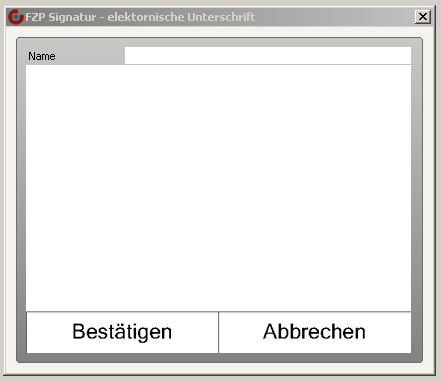
\includegraphics[height=250pt, width=250pt]{steuerelement.PNG}
    \caption[Erfassungsmaske biometrische Unterschrift]{\small{Erfassungsmaske biometrische Unterschrift}}
\end{figure}
\newline
Der blau umrandete Bereich kennzeichnet die Klasse der Erfassungsmaske. Die Erfassungsmaske enthält das geschaffene Steuerelement zur Erfassung der biometrischen Unterschrift. Weiterhin regelt die Maske den Funktionsaufruf zur Speicherung der biometrischen Unterschrift. Ebenfalls wird das Öffnen und Schließen der Erfassungsmaske gesteuert. Der grün umrandete Bereich zeigt die Klasse des Signaturbelegs. Diese dient zum Speichern, Aktualisieren und Laden von biometrischen Unterschrift. Des Weiteren erfolgt eine Prüfung, ob bereits biometrische Unterschrift für den jeweiligen Vorgang vorhanden sind. Darüber hinaus enthält der grüne Bereich eine Klasse mit Funktionen zur Prüfung der Datenbank und deren Version sowie zur Aktualisierung. Die Klasse dient zum Erstellung und Schließen einer Datenbankverbindung. Sie regelt ebenfalls die Ausgabe von Hinweis- und Fehlermeldungen.
\begin{figure}[!ht]
    \centering
    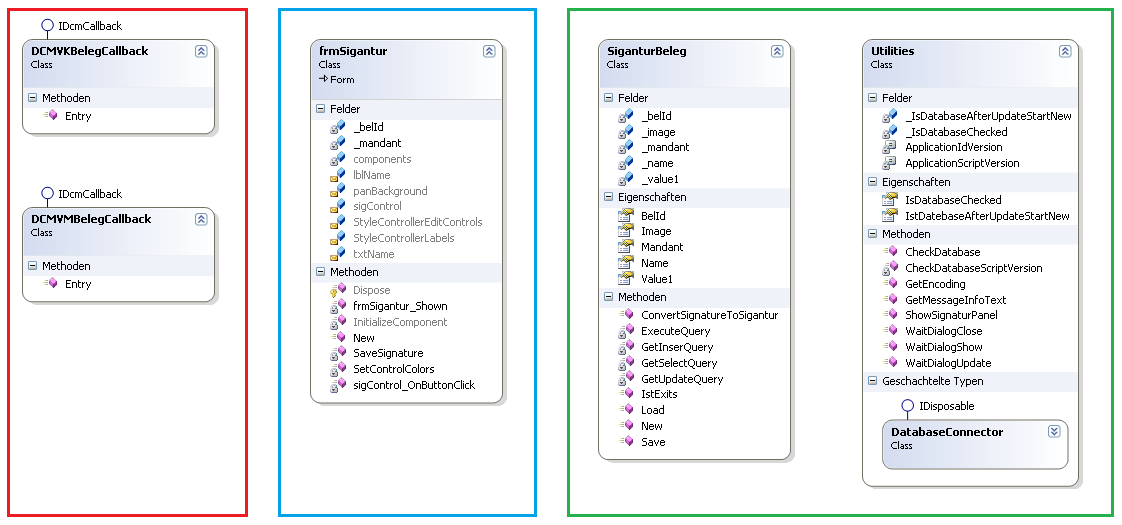
\includegraphics[height=300pt, width=\textwidth]{Klassendiagramm_Abf_Signatur_Edit2.png}
    \caption[Klassendiagramm FZP.OfficeLine.Abf.Signatur]{\small{Klassendiagramm FZP.OfficeLine.Abf.Signatur}}
\end{figure}
\newline
\pagebreak
\textbf{} %Workaround
\newline
Das Klassendiagramm auf der folgenden Seite symbolisert das Projekt "'FZP.Wacom"'. In diesem Projekt wurde im blau umrandeten Bereich das Steuerelement zur Darstellung der biometrischen Unterschrift auf einem Bildschirm geschaffen. Die Funktionen des Steuerelements sind auf der einen Seite die Ermittlung des verwendeten USB bzw. COM-Port des Computers an dem das Signatur-Tablets angeschlossen ist. Auf der anderen Seite wird die Zeichnung des Erscheinungsbilds des Steuerelements, die Entfernung des Unterschriftsbilds vom Display des Tablets und das Schließen des Steuerelements durchgeführt. Die Klassen im grün umrandeten Bereich sind für die folgenden Funktionen zuständig. Das Steuerelement reagiert auf die Eingaben des Signatur-Tablets und leitet diese an die Klassen zur Sammlung, Prüfung und Aufbereitung der Daten aus dem Signatur-Tablet weiter. Danach werden die Daten an die Eingabemaske zur Darstellung weiter geleitet. Abschließend wird mit den aufbereiteten Daten die biometrische Unterschrift erstellt und an die Klasse Signaturbeleg zur Speicherung übergeben.
\begin{figure}[!ht]
    \centering
    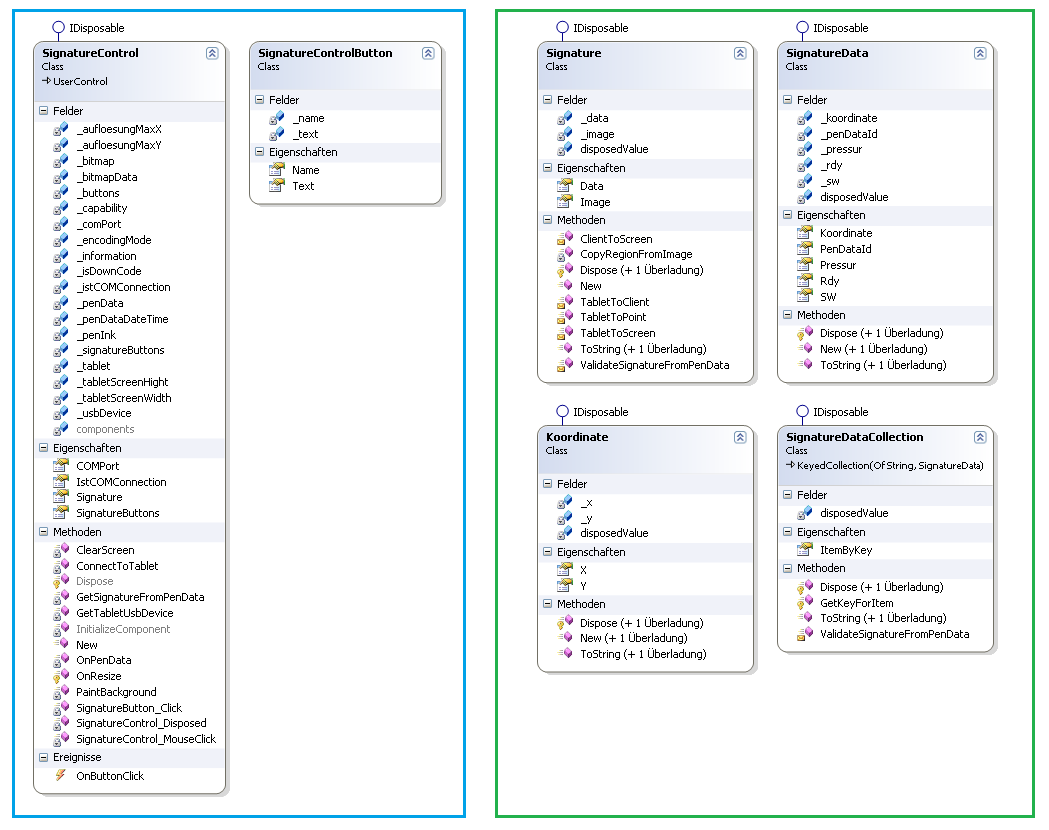
\includegraphics[height=350pt, width=\textwidth]{Klassendiagramm_FZP_Wacom_Edit1.png}
    \caption[Klassendiagramm Erstellung Steuerelement und Aufbereitung Daten]{\small{Klassendiagramm Teilprojekt Erstellung Steuerelement und Aufbereitung Daten}}
\end{figure}
\newline
\pagebreak
\textbf{} %Workaround
\newline
Die Speicherung der Daten erfolgt in der Datenbank der Sage Office Line. Die Sage Office Line benutzt eine MS SQL Datenbank. Die Abkürzung MS SQL steht für Microsoft Structured Query Language und ist ein relationales Datenbankmanagementsystem "'zum Bearbeiten (Einfügen, Verändern, Löschen) und Abfragen von darauf basierenden Datenbeständen"' \cite{sql1} \cite{sql2}. Angesichts dessen ist die Einbindung der neugeschaffenen Datenbanktabellen in das bestehende Datenbankschema problemlos zu bewerkstelligen. Die folgenden Vorteile sind maßgebend für die Nutzung von Microsoft SQL Servern. Die Verwendung von abgespeicherten Verfahrensweisen, d.h. auf einem Server wird Quellcode  gespeichert, der von Anwendungen abgefragt werden kann und zu Performanceverbesserungen von Anwendungen führt. Die Skalierbarkeit, dies bedeutet die Anpassbarkeit an das Wachstum von Unternehmen. Ein MS SQL Server ist für kleine und große Unternehmen gleichmaßen nutzbar, aufgrund der hohen Verarbeitung von Datenbankanfragen. Die Sicherheit wird mittels Benutzerkontensteuerung gewährleistet. Die Benutzerkontensteuerung regelt die Berechtigungen von einzelnen Anwendern bzw. Anwendergruppen sowie deren Eingriffsmöglichkeiten in das System. Zu den Eingriffsmöglichkeiten gehören Lese- und / oder Schreibrechte auf den Datenbanken. Ein weiterer Vorteil ist die Aufzeichnung von Datenbankabfragen, Aktualisierungen und Löschung von Datensätzen mittels Transaktionsprotokollen. Transaktionsprotokolle werden für die Systemwiederherstellung bei fehlerhaften Aktualisierungen oder Löschungen von Datensätzen verwendet. Des Weiteren besitzen MS SQL Server eine automatische Backup Funktion. Hiermit wird eine Kopie der Datenbank sowie der Transaktionsprotokolle auf weiteren Medien erstellt und somit der Schutz vor Datenverlust gesteigert. Als Nachteil von MS SQL Servern können die hohen Lizenzierungskosten sowie der exklusive Installationsort auf Microsoft Betriebssystemen genannt werden. \cite{SQLv1}
%--------------------------------------
% Ergebnisse
%--------------------------------------
\subsection{Ergebnisse}
\label{sec:Ergebnisse}
Das Ergebnis der Datenintegrationsprüfung ist die problemlose Einbindung in das bestehende Datenbankschema. Die Anbindung der Schnittstelle zur Sage Office Line erfolgt mittels DCM-Verfahren sowie die Integration der Formulare in die bestehende Benutzeroberfläche der Sage Office Line ist aufgrund des modularen Aufbaukonzepts von Sage problemlos möglich. DCM heißt ""DLL Common Methode"" und ist eine von Sage geschaffene Methode um externe Schnittstellen mit der Sage Office Line zu verbinden... \textbf{Erklärung DCM + Screenshots + Listings?}

Auf den Screenshots sieht man die fertige Schnittstelle...
%--------------------------------------
% Zusammenfassung
%--------------------------------------
\newpage
\section{Zusammenfassung}
\label{sec:Zusammenfassung}
Der Ausgangspunkt für die Auseinandersetzung mit dem Thema "'Biometrische Unterschrift"' war ein Kundenauftrag. Das Ziel des Kundenauftrags ist die Einführung einer personalisierten Warenabgabe im Bereich Verkauf und Vermietung mittels der Schaffung eines Zusatzmoduls zwischen der Sage Office Line und einem Signatur-Tablet.
\newline
Die Anbindung einer Erweiterung ist hinsichtlich des modularen Aufbaus der Sage Office Line möglich. Die verwendete Technologie in der Softwareentwicklung basiert auf dem Microsoft .NET Framework in Verbindung mit Microsoft Access und dem Microsoft COM Framework. Die Verwaltung der Daten wurde mit einem Microsoft SQL Server realisiert. Die verwendete Technik im Hardwarebereich ist ein Signatur-Tablet der Firma Wacom. Der Einsatz der biometrischen Unterschrift ist angesichts des sofort verfügbaren Nachweises über erbrachte Lieferungen gewählt wurden. Mit der biometrischen Unterschrift werden Daten, wie die Schreibgeschwindigkeit, der ausgeübte Druck, der Bereich und die Dauer der Unterschrift sowie das Schriftbild zur Identifizierung vom Unterzeichner gesammelt und gespeichert. Eine biometrische Unterschrift ist rechtlich bindend und in gerichtlichen Verfahren als Beweismittel anerkannt. 
\newline
Das Ergebnis ist eine voll integrierte Erweiterung in die Sage Office Line. Ein weiteres Ergebnis der Entwicklung ist das wiederverwendbare Steuerelement zur Erfassung der biometrischen Unterschrift. Das Steuerelement kann dadurch in weiteren Zusatzmodulen und Erweiterungen verwendet werden. Ein weiterer Einsatzort wäre in der Lagerverwaltung möglich. Hier wäre die Schaffung eines Zusatzmoduls im Bereich Lagerhaltung und Kommissionierung zur Erfassung der personalisierten Ein- und Auslagerung von Waren und Vermietungsgegenständen denkbar.
%--------------------------------------
% Selbststänigkeitserklärung
%--------------------------------------
\newpage
\section{Selbstständigkeitserklärung}
\normalsize{Ich versichere, dass ich die vorliegende Arbeit ohne fremde Hilfe selbstständig verfasst und nur die angegebenen Quellen und Hilfsmittel benutzt habe. Wörtlich 
oder dem Sinn nach aus anderen
Werken entnommene Stellen sind unter Angabe der Quellen kenntlich gemacht. Die Arbeit wurde bisher in gleicher oder ähnlicher Form weder 
veröffentlicht, noch 
einer anderen Prüfungsbehörde vorgelegt.
\newline
\newline
\newline
\newline
Leipzig, den 16. Juni 2014}
%--------------------------------------
% Quellenverzeichnis
%--------------------------------------
\newpage
%--------------------------------------
% großzügige Formatierungsweise
%--------------------------------------
%\sloppy
\section{Quellenverzeichnis}
\printbibliography[keyword={buch},title={Literatur}]
\printbibliography[keyword={internet},title={Onlinequellen}]

\end{document}